%!TEX root = paper.tex

\section{Introduction} % (fold)
\label{sec:introduction}

Automatic loop invariant inference is a fundamental program analysis problem, 
which is useful in software verification, test-case generation, 
compiler optimization, program understanding, etc. 
In this work, we propose a new framework using machine learning 
to actively learn the loop invariant based on the classification of runtime data. 
By combining selective sampling, support vector machine learning, 
concolic testing and model verification, 
we refine the inferred loop invariant after each iteration 
until it converges and proves the property preserved by the loop program. 

Generally, a loop program $P$ can be written in the following form, 
where $\mathit{Pre}$, $\mathit{Cond}$ and $\mathit{Post}$ are boolean conditions, 
and $\mathit{Body}$ is the loop body. 
\[
    P = \{ \mathit{Pre} \} \mathit{while}(\mathit{Cond}) \{ \mathit{Body} \} \{ \mathit{Post} \}
\]
In practice, the pre-condition $\mathit{Pre}$ is often described by 
the specification documents and checking conditions of the program inputs, 
and the post-condition $\mathit{Post}$ is usually specified 
by assertions and exceptions leading to an error state in the program. 
Let $s = \{ x_1 \mapsto v_1, \ldots, x_n \mapsto v_n \}$ represent 
the evaluation function of the program variables $x_1, \ldots, x_n$
and $\mathit{Body}(s)$ stand for their new evaluation after the execution of $\mathit{Body}$, 
the above program means that (1) $\mathit{Pre}$ is the assumption of $s$; 
(2) if the $\mathit{Cond}$ is satisfied by $s$ at an iteration, 
$\mathit{Body}$ will be executed and $s$ will be updated to $\mathit{Body}(s)$; 
(3) if the $\mathit{Cond}$ is unsatisfied by $s$ at an iteration, 
the while-loop ends and $s$ should satisfy $\mathit{Post}$. 
To prove the correctness of the above program specification, 
we need to find a loop invariant $\mathit{Inv}$ satisfying the following three conditions. 
\begin{align}
    &s \models \mathit{Pre} 
        &&\Rightarrow & s &\models \mathit{Inv} \label{inv:pre} \\
    &s \models \mathit{Inv} \wedge \mathit{Cond} 
        &&\Rightarrow & \mathit{Body}(s) &\models \mathit{Inv} \label{inv:loop} \\
    &s \models \mathit{Inv} \wedge \neg\mathit{Cond} 
        &&\Rightarrow & s &\models \mathit{Post} \label{inv:post}
\end{align}
The goal of this work is developing a method to automatically learn 
the invariant $\mathit{Inv}$ from the loop program and thus prove its correctness. 

\begin{figure}[t]
\begin{subfigure}{0.2\textwidth}
    \centering
    \vspace{0.5cm}
{\scriptsize\begin{verbatim}
void P(int x, int y) {
    assume(x < y);
    while (x < y) {
        if (x < 0) x = x + 7;
        else x = x + 10;
        
        if (y < 0) y = y - 10;
        else y = y + 3; 
    }
    assert(x >= y
        && x <= y + 16);
}
\end{verbatim}}
    \vspace{0.5cm}
    \caption{Loop Program}
    \label{fig:running:example:program}
\end{subfigure}%
\begin{subfigure}{.3\textwidth}
      \centering
      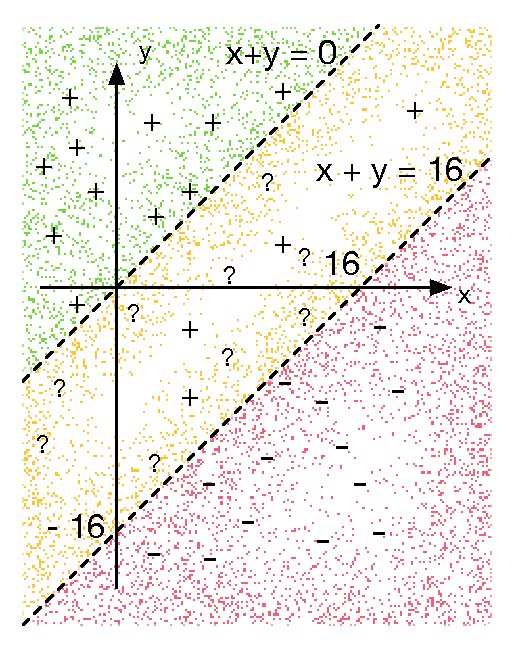
\includegraphics[scale=0.42]{figures/running-sampling.pdf}
      \caption{Sampling}
      \label{fig:running:example:sampling}
\end{subfigure}
\caption{A Running Example}
\label{fig:running:example}
\end{figure}

\begin{figure}[t]
    \centering
    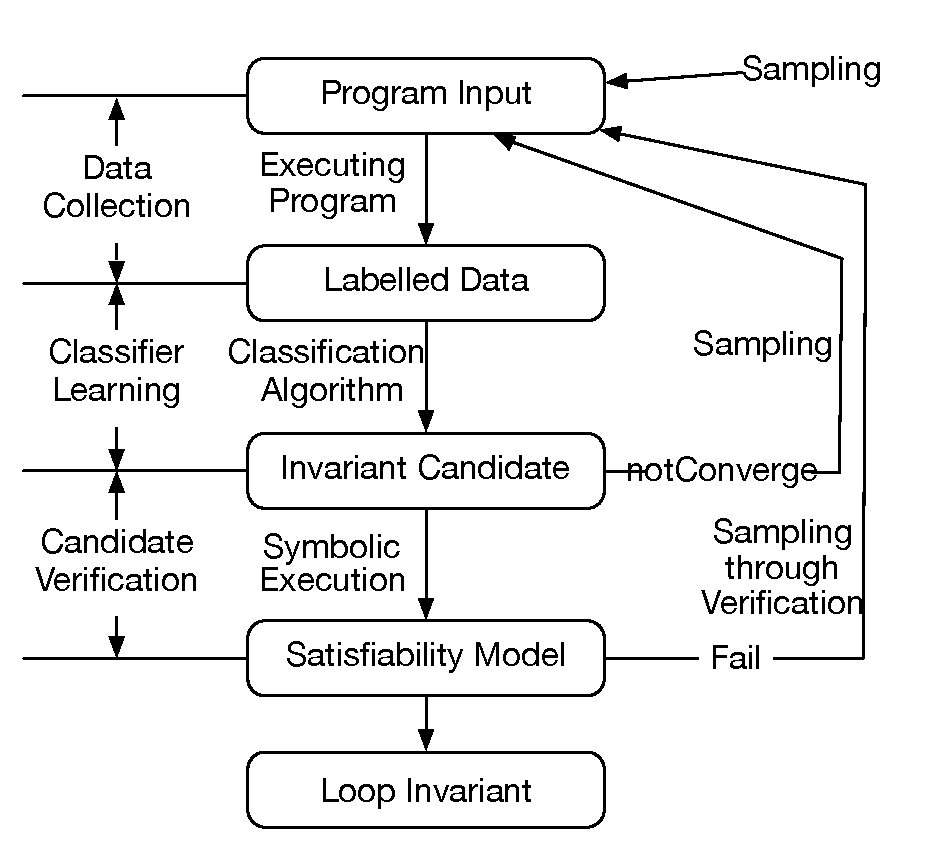
\includegraphics[scale=0.45]{figures/overview.pdf}
    \caption{Loop Invariant Inference Framework Overview}
    \label{fig:overview}
\end{figure}

\medskip\noindent
\textbf{A Running Example}
is shown in Figure~\ref{fig:running:example:program}. 
The loop program $P$ takes two integer variables $x$ and $y$ as inputs. 
The assumption $\mathit{Pre}$ requires that $x < y$, 
which is the same as the loop condition $\mathit{Cond}$. 
When $\mathit{Cond}$ is met in each loop iteration, 
$x$ is increased by $7$ if $x$ is negative, otherwise $x$ is increased by $10$; 
$y$ is decreased by $10$ if $y$ is negative, otherwise $y$ is increased by $3$. 
Finally, the assertion of $P$ requires $y \le x \le y + 16$. 
The correctness of the program specification in Figure~\ref{fig:running:example} 
can be proven by checking the three conditions 
(\ref{inv:pre}), (\ref{inv:loop}) and (\ref{inv:post}) above 
with a loop invariant $\mathit{Inv} = x \le y + 16$ (or $2 \times x \le 2 \times y + 33$, etc). 
We use this running example in the following 
to illustrate different stages of our invariant reference method. 

\medskip\noindent
\textbf{Overview.}
Our framework takes the invariant reference as an active learning and refinement process 
based on iterations of sampling, classification and verification 
as shown in the Figure~\ref{fig:overview}. 
Let $P$ be the loop program. 
\begin{itemize}
    \item 
    % (1)
    In the \textbf{Sampling} stage (see Section~\ref{sec:sampling}), 
    we obtain program inputs from three kinds of sampling sources: 
    random sampling, selective sampling and counter-example sampling. 
    Then, we execute $P$ with these inputs and record $S$ in every loop iteration 
    and label them based on the satisfaction of $\mathit{Pre}$ and $\mathit{Post}$. 
    The regions of different labels can be intuitively shown\footnote{
        The `green' (`yellow' and `red' resp.) areas 
        represent `positive' (`uncertain' and `negative' resp.) samples. 
    } as the areas of different colors in Figure~\ref{fig:running:example:sampling}. 
    When an program input can be found such that 
    $\mathit{Pre}$ is $\mathit{true}$ and $\mathit{Post}$ is $\mathit{false}$, 
    we output it as a proof of the program specification error. 
    \item 
    % (2) 
    Based on $S$ and their labels collected in the \emph{sampling} stage, 
    we \emph{actively} learn the loop invariant as classification models 
    using machine learning algorithms 
    in the \textbf{Classification} stage (see Section~\ref{sec:classification}), 
    e.g., different SVM derivatives. 
    When the recently learnt invariant converges to the previously learnt ones, 
    we treat it as a invariant candidate and move to the verification step. 
    Otherwise, we apply selective sampling on the recently learnt invariant 
    to add more samples in the sampling stage. 
    When a sample cannot be classified using a certain classification model, 
    we try other alternative models in a sequential order. 
    \LL{We prove the termination of the \emph{classification} stage if such an invariant exists.}
    \item 
    % (3) 
    When an invariant candidate is found, 
    we check its correctness in the \textbf{Verification} stage (see Section~\ref{sec:verification}). 
    First, we insert the candidate into the loop program and generate all the program execution traces 
    based on concolic testing using KLEE. 
    Then, we verify three loop invariant conditions 
    with respect to all of the program execution traces (i.e., different $\mathit{Body}$) 
    using a SMT solver (e.g., Z3 in this work). 
    If the verification is successful, we claim the correctness of $P$ and output the loop invariant. 
    Otherwise, we add the counter-example from Z3 as a new sample 
    and restart from the \emph{sampling} stage. 
\end{itemize}

\medskip\noindent
\textbf{Contributions.}
Our contributions are four-fold. 
\begin{itemize}
    \item 
    We are the first to propose an active learning and refinement framework 
    for automatic invariant inference based on machine learning. 
    Since the samples are chosen for clear purpose 
    to refine the invariant candidate in the \emph{sampling} stage, 
    the invariant converges efficiently. 
    Furthermore, because the counter-examples generated in the \emph{verification} stage 
    give very accurate information to amend the invariant candidate, 
    they become a useful supplementary to overcome the weakness of machine learning 
    and fine-tune the invariant candidate. 
    \item 
    Our framework is highly adaptable to different invariant inference scenarios 
    because the classification methods have a wide range of choices. 
    In this work, we show that linear, polynomial as well as 
    their conjunctive classification methods work effectively in our framework. 
    More importantly, our framework can be easily and intuitively extended with other alternative methods. 
    \item 
    Our framework can be practically used to verify real programs with ease, 
    as our framework is language- as well as platform-independent 
    based on the samples generated at runtime. 
    In this work, we choose GSL for selective sampling, LibSVM for SVM classification, 
    Z3 for invariant verification and KLEE for concolic testing. 
    They can be replaced by any other COTS libraries and tools, 
    whenever the desired functionalities are provided. 
    \item 
    We implement our framework as a tool called \textsc{Zilu} 
    and compare it with other available state-of-the-art invariant inference tools, 
    i.e., CPAChecker, Interproc. 
    Our experiment results show that 
    we are the only tool that can work with polynomial invariant inference. 
    Notice that the polynomial invariant inference works in our framework 
    naturally with very light additional programming. 
    % Based on the design of different approaches,
    % we also claim that our framework have better extensibility comparing with their method.
\end{itemize}

\medskip\noindent
\textbf{Structure of this paper.}

% section introduction (end)